\documentclass{uc3mpracticas}

\usepackage{helvet}
\usepackage{multicol}
\renewcommand{\familydefault}{\sfdefault}
\usepackage{changepage}
\usepackage{geometry}
\usepackage{caption}
\usepackage{xcolor,colortbl}
\usepackage{makecell}

\usepackage{amsfonts}

\definecolor{Gray}{gray}{0.85}
\definecolor{LightCyan}{rgb}{0.88,1,1}
\definecolor{LightGreen}{rgb}{0.29,1,0.39}

\newcolumntype{g}{>{\columncolor{Gray}}l}
\newcolumntype{b}{>{\columncolor{LightCyan}}c}


%%%%%%%%%%%%%%%%%%%%%%%%%%%%%%%%%%%%%%%%%%%%%%%%%%%%%%%%%%%%%%%%%%%%%%%%%%%%%%%%
%%%                   Plantilla Prácticas UC3M                               %%%
%%%                Universidad Carlos III de Madrid                          %%%
%%%                   Alejandro Valverde Mahou                               %%%
%%%%%%%%%%%%%%%%%%%%%%%%%%%%%%%%%%%%%%%%%%%%%%%%%%%%%%%%%%%%%%%%%%%%%%%%%%%%%%%%

%Permitir cabeceras y pie de páginas personalizados
\pagestyle{fancy}

%Path por defecto de las imágenes
\graphicspath{ {./images/} }

%Declarar formato de encabezado y pie de página de las páginas del documento
\fancypagestyle{doc}{
  %Cabecera
  \headerpr[1]{Test de Primalidad - AKS}{}{Teoría Avanzada de la Computación}
  %Pie de Página
  \footerpr{}{\textbf{UC3M}}{{\thepage} de \pageref{LastPage}}
}

%Declarar formato de encabezado y pie del título e indice
\fancypagestyle{titu}{%
  %Cabecera
  \headerpr{}{}{}
  %Pie de Página
  \footerpr{}{}{}
}


\appto\frontmatter{\pagestyle{titu}}
\appto\mainmatter{\pagestyle{doc}}


\begin{document}
  %Comienzo formato título
  \frontmatter


  %Portada 1 (Centrado todo)
  \centeredtitle{Images/LogoUC3M.png}{Grado en Ingeniería Informática}{Curso 2020/2021}{Teoría Avanzada de la Computación}{Test de Primalidad}{\textit{AKS}}

  \vspace{55mm}

  \authors{Iván Miguelez García}{100383387}{Alba Reinders Sánchez}{100383444}{Alejandro Valverde Mahou}{100383383}{}{}

  \newpage

  %Índice
  \tableofcontents

\newpage

  %Comienzo formato documento general
  \mainmatter

  \begin{abstract}
    En este trabajo se realiza un estudio del algoritmo de test de primalidad \textit{AKS} desde una perspectiva analítica y empírica. Se plantea hacer el estudio dividiendo en distintas partes el algoritmo para calcular el coste computacional de cada parte.

    \vspace{2mm}

    El estudio se hará sobre el código proporcionado en la práctica, que se encuentra en el lenguaje de programación \textit{Java}. Además, se propone una traducción a \textit{Python}, para facilitar su comprensión.

  \end{abstract}



  \newpage

  \section{Introducción}

  Para estudiar la complejidad computacional del algoritmo \textit{AKS} se ha dividido el estudio en 3 hitos diferentes: \textit{Heurísticas iniciales}, \textit{cálculo del Totient} y \textit{análisis de la condición suficiente}.

  \vspace{2mm}

  El documento se divide en 3 secciones principales, una para cada hito que se ha realizado. De cada hito se realiza el análisis analítico y empírico de la parte correspondiente en el código de \textit{AKS} que se proporciona.

  \vspace{2mm}

  Para los cálculos empíricos realizados, se han escogido aleatoriamente 500 números primos entre 5 y 9 cifras, 100 números por cada cifra.


  \section{Hito 1: Heurísticas iniciales}

  Para esta primera parte de la práctica se pide realizar un estudio analítico y empírico de las dos primeras heurísticas del algoritmo \textit{AKS}, utilizado para determinar la primalidad de un número natural.

  \vspace{2mm}




  \subsection{Heurística 1: comprobación potencia perfecta}

  La primera heurística consiste en comprobar si un número es una potencia perfecta. Para ello, se debe cumplir la siguiente propiedad.

  $$ a^b = n \; | \; a, b \in \mathbb{N}, \; b>1$$

  Si esta propiedad se cumple, se puede afirmar que $n$ no es un número primo.


  \subsubsection{Estudio analítico}
  Se pretende determinar la complejidad temporal de los pasos del algoritmo en los que se lleva a cabo esta primera tarea. A continuación, se realiza el estudio analítico para averiguar \textit{T(n)} y \textit{O(n)}.

  \vspace{2mm}

  Para ello se tiene que analizar la estructura del código. Se puede ver que está compuesto por dos bucles \textit{do while}. El bucle exterior itera sobre $a$ y el bucle interior itera sobre $b$.

  \vspace{2mm}

  Para el análisis del bucle exterior, es necesario determinar el valor máximo de $a$.
  Se puede afirmar que, dado que el valor mínimo de $b$ es 2, el valor máximo de $a$ será $\sqrt{n}$, porque:

  $$ a^2 = n \; \Rightarrow \; a = \sqrt{n} $$

  El bucle interior requiere un desarrollo un poco mayor. Para conseguir el número de iteraciones es necesario despejarlo en la ecuación.

  \vspace{2mm}

  $$ a^{\frac{\log n}{\log a} - 1 + k} > n \Rightarrow \log a^{\frac{\log n}{\log a} - 1 + k} > \log n \Rightarrow (\frac{\log n}{\log a} - 1 + k) * \log a > \log n \Rightarrow  \frac{\log n}{\log a} - 1 + k > \frac{\log n}{\log a}$$

  $$ -1 + k > 0 \Rightarrow k > 1 $$

  Por tanto, el número de ciclos del bucle interior será 3 (Tiene que recorrer $k=0$, $k=1$ y $k=2$)

  \vspace{2mm}

  Si se unen ambas complejidades, se puede ver que para esta primera heurística, la complejidad temporal es:

  $$ T(n) = \displaystyle 3*\sqrt{n}$$

  Y el coste computacional es:

  $$ O(n) = \sqrt{n}$$


  \subsubsection{Estudio empírico}\label{empirico}

  Como se puede ver en la Figura \ref{fig:h1}, los tiempos obtenidos coinciden con la complejidad esperada. La complejidad de la heurística es $ O(n) = \sqrt{n} $, y haciendo uso de un optimizador de parámetros, se obtiene una curva con valor:

  $$ 1.7654419^{-07} * \sqrt{n} $$

  % \begin{itemize}
  %   \item Puede ser que no se hayan probado con números suficientemente grandes como para apreciar la curva esperada.
  %   \item Puede que el resultado esperado no esté escalado correctamente, y por tanto los valores no coincidan.
  %   \item Debido a que se ha ejecutado un código en \textit{Java} en una máquina \textit{Windows}, puede que los tiempos no estén bien medidos y tengan mucho ruido,
  % \end{itemize}
  %
  % Para próximos hitos se volverá a probar, pero con una cantidad de números mayor.

  \begin{figure}[!h]
    \centering
    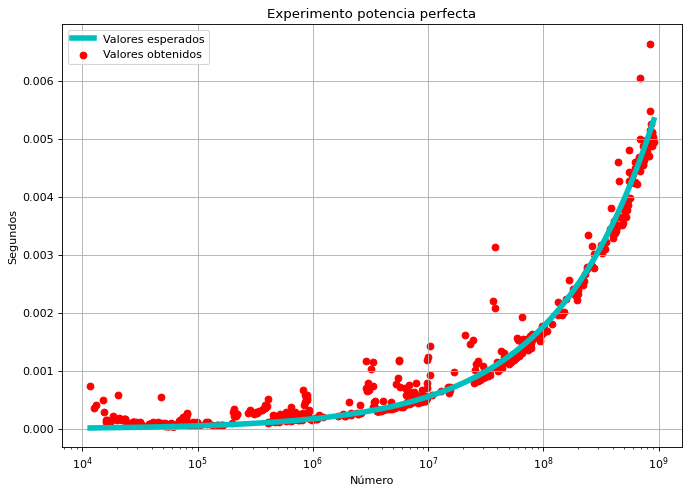
\includegraphics[width=.8\linewidth]{./Images/h1.png}
    \caption{Gráfica de tiempo de la Heurística 1}
    \label{fig:h1}
  \end{figure}

  Aún así se observa cierto ruido por realizar la ejecución en \textit{Windows}, ya que se producen a la vez otros procesos ajenos que pueden influenciar en los tiempos del estudio y por tanto generar en la gráfica puntos que no se ajustan a la complejidad calculada.




  \subsection{Heurística 2: cálculo de \textit{r} y \textit{mcd}}

  Esta segunda heurística consiste en comprobar si se cumple la siguiente premisa:

  $$ \exists a \leq r \mid 1 < mcd(n,a) < n $$

  Si se cumple, se dice que $n$ es un número compuesto.


  \subsubsection{Estudio analítico}
  Para determinar la complejidad temporal de esta segunda tarea se tiene que dividir el estudio en dos partes. En primer lugar, se debe calcular $r$ y después calcular el $mcd$.

  \vspace{4mm}

  \textbf{Cálculo de \textit{r}}

  \vspace{2mm}


  Analizando la estructura del código, se ve que está compuesto por un bucle \textit{do while} que itera sobre $r$ y que dentro se llama a la función \textit{multiplicativeOrder()}. Esta función tiene a su vez un bucle \textit{do while} que itera sobre $k$.

  \vspace{2mm}

  Se busca el mínimo $r$ tal que:

  $$ O_r(n) > \log_2^2(n) $$

  Donde $O_r(n)$ es el orden de $n$ módulo $r$ y representa el menor $k$ tal que:

  $$ O_r(n) = k \; \Leftrightarrow \; n^k \equiv 1 \; mod \; r$$


  Se sabe cuál es el máximo $r$ por el lema 4.3 de \textit{Primes is in P}\cite{primesinp}:

  $$ r \leq \lceil \log^5(n) \rceil $$

  Por lo tanto se concluye que la complejidad temporal del cálculo de $r$ es la unión de las complejidades de ambos bucles:

  $$ T(n) = \log^5(n) * \log^2(n) = \log^7(n) = O(n)$$

  \vspace{2mm}

  \textbf{Cálculo del \textit{mcd}}

  \vspace{2mm}

  Por último, para la complejidad de calcular el máximo común divisor de dos número $a$ y $b$, se tiene en cuenta el peor de los casos: cuando $a$ y $b$ son números consecutivos en la sucesión de \textit{Fibonacci}.

  \vspace{2mm}

  En este caso, el número de iteraciones del bucle es el índice del término de la sucesión, el cual se saca con la fórmula de E.Lucas:

  $$ f_n =\frac{\phi^n - (1-\phi)^n}{\sqrt{5}} $$

  cuya complejidad es $\log(n) $ porque es un cálculo directo que no hace uso de bucles.

  \vspace{2mm}


  Por tanto, la complejidad total del $mcd$:

  $$ T(n) = \log(n) * \log^5(n) = \log^6(n) = O(n)$$

  y la fórmula de la complejidad total de la heurística 2 es de:

  $$ T(n) = \log^7(n) + \log^6(n)$$

  $$ O(n) = \log^7(n)$$




  \subsubsection{Estudio empírico}

  En este caso, tal como se puede ver en la Figura \ref{fig:h2}, la diferencia entre el tiempo propuesto en el estudio analítico y el empírico es mucho mayor. Esto puede indicar que los cálculos del estudio analítico no sean correctos, o puede deberse a las mismas causas que se han descrito en el anterior estudio empírico \ref{empirico}.

  \begin{figure}[!h]
    \centering
    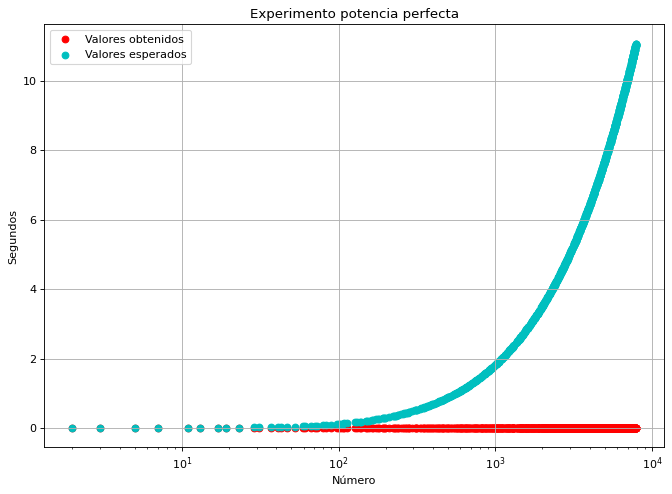
\includegraphics[width=.8\linewidth]{./Images/h2.png}
    \caption{Gráfica de tiempo de la Heurística 2}
    \label{fig:h2}
  \end{figure}


  \section{Hito 2: Cálculo del Totient}

  En esta segunda parte se pide realizar el estudio analítico y empírico del cálculo del \textit{Totient} ($\phi(r)$). Donde $\phi(r)$ es el número de enteros positivos más pequeños o iguales que $r$ tales que $r$ es coprimo con ellos, es decir, su $mcd$ es 1.



  \subsection{Estudio analítico}

  A continuación, se realiza el estudio analítico para averiguar la complejidad temporal del algoritmo. Analizando el código se ve que la función del cálculo del \textit{Totient} está formada por un bucle \textit{for} externo y un bucle \textit{while} interno:

  \vspace{2mm}

  El bucle de fuera se ejecuta como mucho $\sqrt{r}$ veces, dado que en este caso, la peor situación se da cuando $r$ es un número primo, y por tanto el bucle de fuera tiene que recorrer desde $i = 2$ hasta $i = \lfloor \sqrt{n} \rfloor + 1$. Simplificando, se encuentra en $\sqrt{r}$ veces.

  \vspace{2mm}

  El bucle de dentro se ejecuta como mucho $\log{r}$ veces, porque el peor caso resulta cuando $ r = i^k $ donde $ k $ es un número entero e $ i $ representa el iterador del bucle. Por tanto, despejando, $k = \log_ir$, y $k$ representa el número de veces que se realiza el bucle.

  \vspace{2mm}

  Para que se cumpla el peor de los casos del bucle \textit{for} exterior, $r$ tiene que ser un número primo, y por tanto el bucle \textit{while} interior no se realizará ninguna vez. En el caso de que $r$ sea el número primo, también se obtiene el valor máximo de $\phi(r)$, que es $r-1$.

  \vspace{2mm}

  La complejidad temporal de este apartado es por tanto:

  $$ T(r) = \sqrt{r-1} * \log r $$

  $$ O(r) = \sqrt{r} * \log r $$

  y dado que la complejidad de $r$ es $\log^5(n)$, la complejidad es:

  $$ O(n) = \sqrt{\log^5(n)} * \log (\log^5(n)) $$

  \section{Hito 3: Análisis de la condición suficiente}

  \section{Conclusiones}


  \newpage

  \bibliographystyle{unsrt}
  \bibliography{bibliography}



\end{document}
